\section{GAA(Gate-All-Around)構造}
GAA(Gate-All-Around)構造は、チャネルを全周囲からゲート電極で包み込むことにより、静電制御性を極限まで高めたデバイス構造である。  
従来のFinFETではゲートが三方向からチャネルを制御していたのに対し、GAAはチャネルの上下方向にもゲート電界が作用するため、  
チャネルポテンシャルの均一性が飛躍的に向上し、ドレイン電界の侵入がほぼ完全に抑制される。  
この結果、短チャネル効果(SCE)およびドレイン誘起バリア低下(DIBL)がさらに低減され、  
しきい値電圧$V_{\mathrm{th}}$の安定性とサブスレッショルドスイング(SS)の改善が達成される。

ナノシート型GAA構造では、複数のチャネル層(Nanosheet)を垂直方向に積層し、それぞれを独立にゲートで包囲する。  
この積層構造により、面積効率を維持しつつ実効チャネル幅を拡大できる。  
有効チャネル幅$W_{\mathrm{eff}}$はFinFET構造に対して次式で表される:
\begin{equation}
W_{\mathrm{eff}} = 2n(H + W),
\end{equation}
ここで$n$はチャネル層数、$H$はシート厚、$W$はチャネル幅である。  
この式が示すように、GAAではFinFETと異なり上下両面の電流経路が追加されるため、同一フットプリントに対してより高い駆動能力を実現できる。

さらに、GAA構造は「構造的なスケーラビリティ」を備えており、チャネル幅$W$を減少させつつ層数$n$を増やすことで、  
電気的特性を維持したまま幾何学的スケーリングを継続できる。  
この特性により、IMECやSamsungをはじめとする研究機関・メーカーでは、5\,nm世代以降でのGAA採用を加速させ、  
1.4\,nmクラスのノードにおいてもチャネル制御性と電流駆動性能の両立が実現されつつある。

一方で、ナノシートの積層・分離工程には高い製造精度が要求される。  
層間酸化膜の厚さ均一性、ゲート堆積時の段差被覆性、およびチャネル層のエッチング選択性が信頼性に直結する。  
これらの課題に対処するため、Selective Epitaxial Growth(SEG)によるチャネル形成や、Atomic Layer Deposition(ALD)によるゲート絶縁膜制御技術が導入されている。

GAAは、FinFETの静電制御を限界まで拡張した「完全電界包囲デバイス」として、次世代スケーリングの中核技術となっている。  
次章では、n型およびp型デバイスを垂直方向に積層したCFET(Complementary FET)構造について、その統合設計思想と課題を論じる。

\begin{table}[t]
  \centering
  \caption{GAA(Gate-All-Around)ナノシート構造の代表パラメータ\\
  Representative Parameters of GAA Nanosheet Structure}
  \label{tab:gaa_params}
  \setlength{\tabcolsep}{3pt}       % 列間やや広く
  \renewcommand{\arraystretch}{1.15}% 行間ゆとり
  \small                            % 通常より少し小さめ(視認性確保)
  \resizebox{\columnwidth}{!}{      % 幅は自動で調整
  \begin{tabular}{lccc}
    \toprule
    パラメータ & 記号 & 代表値 & 備考 \\[-3pt]
    Parameter & Symbol & Typical Value & Remarks \\
    \midrule
    ナノシート層数 & $n$ & 3--5 &
      \begin{tabular}[c]{@{}l@{}}積層により有効チャネル幅$W_\mathrm{eff}$が増大\\
      Stacking increases $W_\mathrm{eff}$\end{tabular} \\
    シート厚 & $T_s$ & 5--8\,nm &
      \begin{tabular}[c]{@{}l@{}}チャネル厚制御が性能を支配\\
      Channel thickness dominates performance\end{tabular} \\
    シート間距離 & $S$ & 10--12\,nm &
      \begin{tabular}[c]{@{}l@{}}熱干渉と寄生容量に影響\\
      Affects thermal and parasitic coupling\end{tabular} \\
    有効チャネル幅 & $W_\mathrm{eff}$ & $2n(H+W)$ &
      \begin{tabular}[c]{@{}l@{}}全包囲ゲート寄与を反映\\
      Reflects all-around gate contribution\end{tabular} \\
    しきい値電圧 & $V_\mathrm{th}$ & 0.35--0.40\,V &
      \begin{tabular}[c]{@{}l@{}}対称構造で制御容易\\
      Symmetric structure allows easy control\end{tabular} \\
    サブスレッショルド特性 & $SS$ & 60--65\,mV/dec &
      \begin{tabular}[c]{@{}l@{}}理想スイングに近似\\
      Near-ideal subthreshold swing\end{tabular} \\
    電流駆動比 & $I_\mathrm{ON}/I_\mathrm{OFF}$ & 2--3× &
      \begin{tabular}[c]{@{}l@{}}FinFET比で高駆動効率\\
      2–3× drive gain over FinFET\end{tabular} \\
    \bottomrule
  \end{tabular}
  } % end resizebox
\end{table}

% =====================================================
% Fig. 6 : GAA(Gate-All-Around)ナノシート構造 断面図
% =====================================================
\begin{figure}[t]
  \centering
  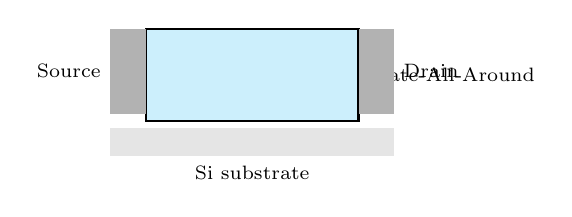
\begin{tikzpicture}[scale=0.9, every node/.style={font=\scriptsize}]
    % substrate
    \fill[gray!20] (0,0) rectangle (4,0.4);
    \node[below] at (2,0) {Si substrate};

    % nanosheets (3層)
    \foreach \y in {0.6,1.0,1.4} {
      \fill[orange!30] (0.8,\y) rectangle (3.2,\y+0.2);
      \draw[black!50] (0.8,\y) rectangle (3.2,\y+0.2);
    }

    % gate stack
    \draw[thick,fill=cyan!20] (0.5,0.5) rectangle (3.5,1.8);
    \node[right] at (3.55,1.15) {Gate-All-Around};

    % source/drain
    \fill[gray!60] (0,0.6) rectangle (0.5,1.8);
    \fill[gray!60] (3.5,0.6) rectangle (4.0,1.8);
    \node[left] at (0,1.2) {Source};
    \node[right] at (4,1.2) {Drain};
  \end{tikzpicture}

  \caption{GAAナノシート構造の模式断面図(S/D領域とゲート包囲面を示す)\\
  \footnotesize Schematic cross-section of GAA nanosheet structure showing gate wrapping around multiple stacked channels.}
  \label{fig:gaa_cross}
\end{figure}

